\noindent
Graph processing is a critical component in a broad range of applications ranging from  social network analysis, medical diagnostics, and drug interaction studies.  Given the vast size of these graphs with billions of edges and vertices, graph algorithms stress memory and scaling capabilities of computing systems. In this proposal we treat graph algorithms as linear algebraic problem formulations, where graphs are represented as adjacency matrices.  The evolving duality between graph algorithms and their equivalent matrix operations forms a solid basis for designing computing systems that can efficiently manipulate matrix operations.  For example, there are well known linear algebraic problem formulations for graph algorithms such as breadth first search, strongly connected components, shortest path, stress centrality, betweenness centrality,  sub-graph detection and so on.  These algorithms demand a diverse range of matrix manipulations, including matrix multiplication, Kronecker product,  matrix decomposition, inner and outer products, matrix inversion, matrix transpose and Eigen value computation.  Supporting such a broad range of operations on extremely large matrices is the first challenge that will be tackled in this proposal. 

%An equally daunting challenge is the representation of large graphs as adjacency matrices in memory.
Given the diversity of application domains where graph analytics may be used, the structure of graphs may also be varied. To improve storage and bandwidth efficiency sparse graphs may be stored in  (double) compressed sparse row (CSR) and column (CSC) formats. But sparse graph representations also worsen irregular access patterns to memory. Some graphs may exhibit power law distributions where only a few vertices contribute to most edges in the graph. Such disparity leads to significant load imbalances in computations.  Efficiently handling both sparse and dense matrices with varying degrees of connectivity is the second challenge tackled in this proposal. 
 
Finally, scaling the execution of linear algebraic manipulations, through parallelization, while mitigating Amdahl's bottleneck is the last challenge that this proposal tackles. Parallel execution of matrix operations can be mapped to various distributed computing paradigms, such as Mapreduce, Pregel and Parallel-R. For instance, many PGAS (partitioned global address space) approaches distribute equal number of vertices across nodes (equal number of rows from the adjacency matrix). 
But when vertex degrees exhibit power law distribution it  is extremely difficult to balance the load across computational nodes. Launching a  new iteration of the computation  requires the previous iteration to complete, thereby forcing a barrier synchronization across various threads. In the presence of load imbalances such synchronizations curtail scaling. 

These observations lead to the main research thrusts of this proposal, as described below. To guide the discussion of the proposed research we present an overview of the system architecture that we will design and build. The system will rely on processing-in-memory architecture, but appropriately adopted for matrix manipulations used in graph processing. Figure~\ref{fig:arch} present the overview of the architecture . The basic building block of the GAMA (graph acceleration through matrix abstraction) system is a GAMA corelet, which is a 16-wide SIMD pipeline that is optimized by vector multiply-accumulate operations. Each corelet is provisioned with \emph{Elastic} L1 cache.  32 corelets are placed on a single die and share a single large L2 cache designed using eDRAM. The L2 cache is then backed up by 4X8GB DiRAM4 memory modules. DiRAM4 is a die-stacked DRAM die that is provided by Tezzaron (one of our service providers in this project). The 32 corelets are 2.5D stacked with DiRAM4. This entire package is called a GAMA tile. We will integrate 16 GAMA tiles to create the whole GAMA accelerator system. 16 GAMA tiles are interconnected  using our custom-designed 1Tbps inter-tile interface. The GAMA system is interfaced with IBM Power8-based host system using OpenCAPI interface. 

At each layer of the above design we propose several innovative ideas. At the corelet layer we propose to design specialized address mapping engines that translate the sparse matrix indices to generate the row/column index of matrix elements based on the underlying sparse matrix format. While the 32 GAMA corelets can do MIMD computations they can  be dynamically reconfigured to execute a single instruction across a very wide vector range when accesses are highly sequential.  The elastic  cache attached to each corelet is architected to support both dense/sequential and sparse/random accesses to a matrix. The elastic cache is a low-overhead cache organization that supports variable width cache lines to improve cache usage efficiency.  
 The unique aspect of DiRAM4 memory, compared to other competing memories such as high bandwidth memory, is that each DiRAM4 die supports more channels per die, but uses narrow width channels. Such a design is well suited for graph workloads that need narrow width memory level parallelism. The narrow width channels can be reconfigured to create a single wide width channel to support dense matrices. The memory layer itself is made semantically aware of the matrix structure and its preferred lay out and access patterns in memory. The semantic awareness comes from application provided hints that are conveyed to the memory controller through APIs. Since graphs that are spread over multiple tiles demand high bandwidth inter-tile access. High-bandwidth links  posing power, thermal, and signal integrity challenges.  We tackle this challenge with various charge-based and injection-locking techniques for high-speed links. The scalability of parallel graph algorithms will be improved by enabling barrier elision hardware that can be used by the application developer to tradeoff accuracy with latency. We provide an in-depth visibility to software to monitor changes to the graph structure and take action to deal with potential load imbalances.  
\begin{figure}
\center
%\vspace{-8ex}
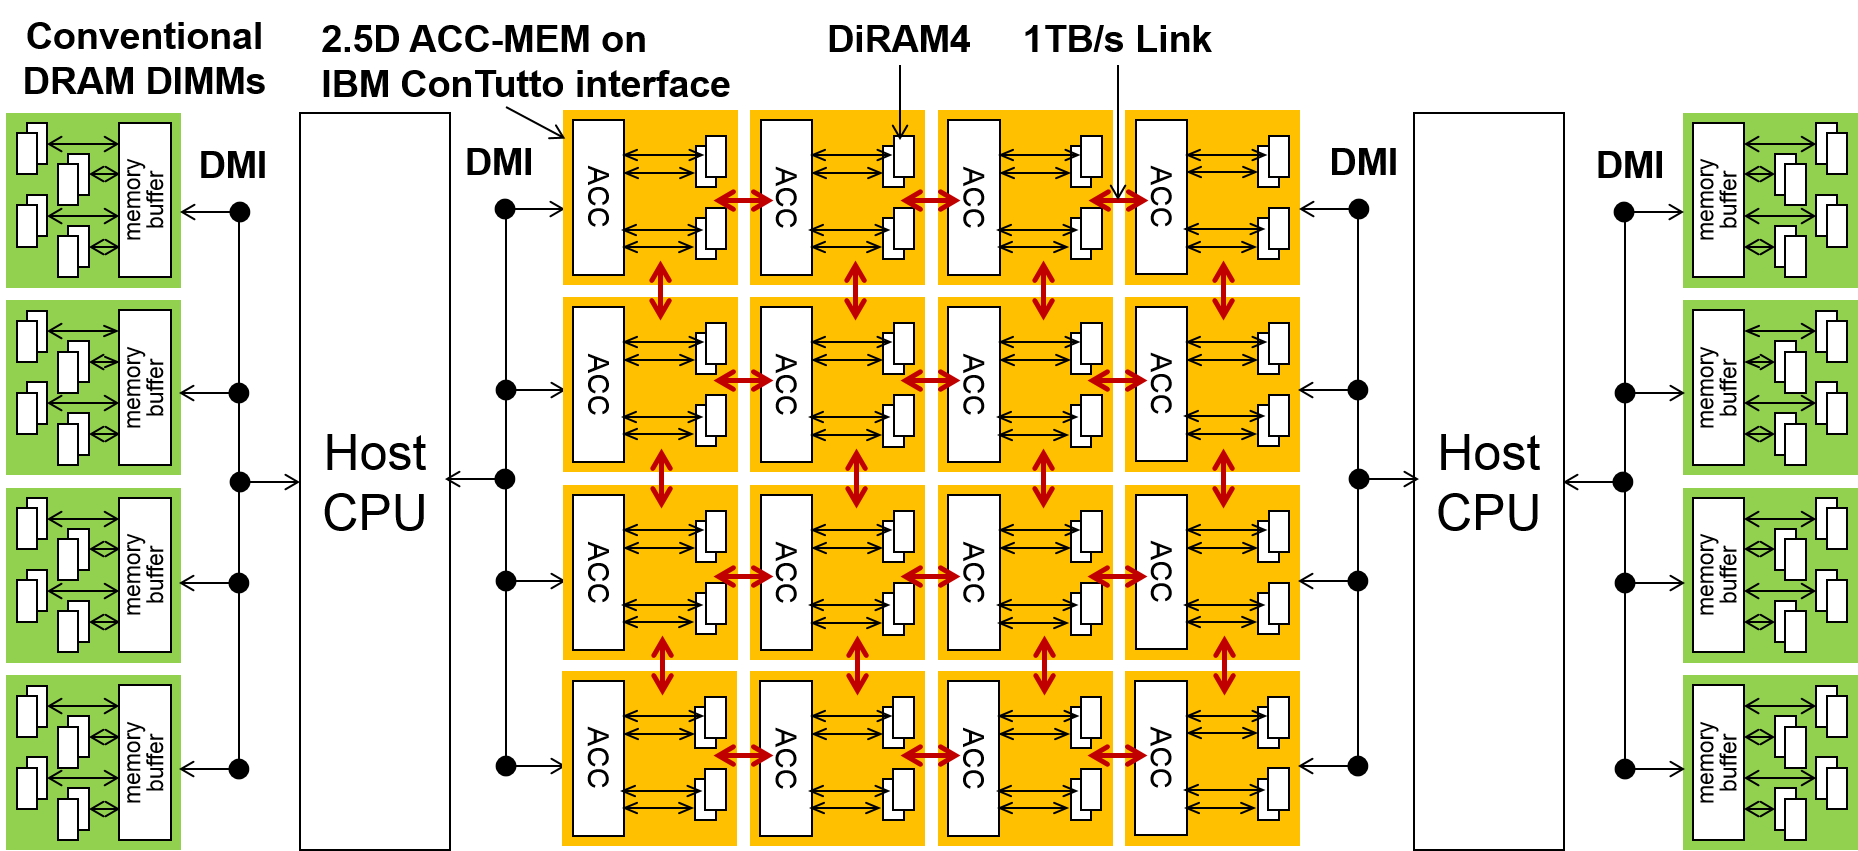
\includegraphics[width=1.0\linewidth]{fig/arch.png}
\caption{GAMA System Architecture}
\label{fig:arch}
\end{figure}


\begin{comment}


\noindent 
To guide the discussion of the proposed research we present an overview of the system architecture that we will design and build. The system will rely on processing-in-memory architecture, but appropriately adopted for matrix manipulations used in graph processing.   Figure~\ref{fig:arch} present the overview of the architecture. The GAMA (graph acceleration through matrix abstraction) system consists of 16 tiles; and each tile, called the GAMA tile,  consists of a GAMA core closely tied to four 8GB DiRAM4 dies. DiRAM4 is a die-stacked DRAM die that is provided by Tezzaron (one of our service providers in this project). The unique aspect of DiRAM4 compared to other competing memories, such as high bandwidth memory, is that each DiRAM4 die supports more channels per die, but uses narrow width channels. Such a design is well suited for graph workloads that need memory level parallelism to access multiple vertices concurrently. We will use 2.5D integration for stacking GAMA core with DiRAM4 die thereby supporting 4TB/s aggregate in-package bandwidth per tile.  16 GAMA tiles are clustered together using 1TB/s inter-tile interface to form the full GAMA system. 

Each GAMA tile is  built as an SMX2 form factor accelerator board which is interfaced to a IBM Power8-based host system using OpenCAPI interface. We will rely on  the OpenPOWER mother board which provides OpenCAPI interface through SMX2 sockets.  Traditionally IBM Power8 supported 8 DMI (differential memory interface) links  to connect to external memory. Recently IBM demonstrated ConTutto Card design for integrating an FPGA accelerator into P8 by plugging into one of the DMI links. We will be using the same approach to design a single GAMA tile card that will be integrated into a DMI link. Two IBM Power8 hosts will be used and each host will connect to eight GAMA tiles.  IBM will be providing the services for enabling OpenCAPI interface on each GAM tile. IBM will also be building a custom board that is based on OpenPOWER design. 
The OpenPOWER mother board provides OpenCAPI interface through SMX2 sockets that will host the GAMA tiles. The board enables up to 16 SMX2 tiles connected either to OpenPOWER cores or among themselves. The GAMA  system is interfaced with the memory channel of a host CPU using the OpenCAPI providing up to 8 memory channels per GAMA system.

Although CAPI provides coherent memory interface to the accelerators, in this proposal the memory space associated with the GAMA system is a non-cacheable region to  eliminate the need for managing cache coherence between caches of the host systems and GAMA tiles. 

Each GAMA core consists of 32 MIMD-style corelets each with three separate \emph{elastic} L1 caches. The elastic cache is a specialized cache organization that supports variable width cache lines to improve cache usage efficiency.  As such the elastic L1 caches are architected to support both dense/sequential and sparse/random accesses.
Furthermore,  all the corelets share a elastic turbo-boosted eDRAM cache which acts as an L2 cache. 

Corelets support a reconfigurable execution pipeline that is designed for doing various matrix operations in an ASIC flow. For instance, a single fused floating point multiply-accumulate operation across a sparse row and a sparse vector may be configured to find the single hop neighbors of a given vertex, which is typically one iteration of a breadth first search algorithm. %NAM: WHAT ARE THE OTHER OPERATIONS THAT YOU ENVISION? I AM NOT SURE IF MATRIX OPERATIONS HAVE MUCH OF ANYTHING ELSE.  

\begin{figure}
\center
%\vspace{-8ex}
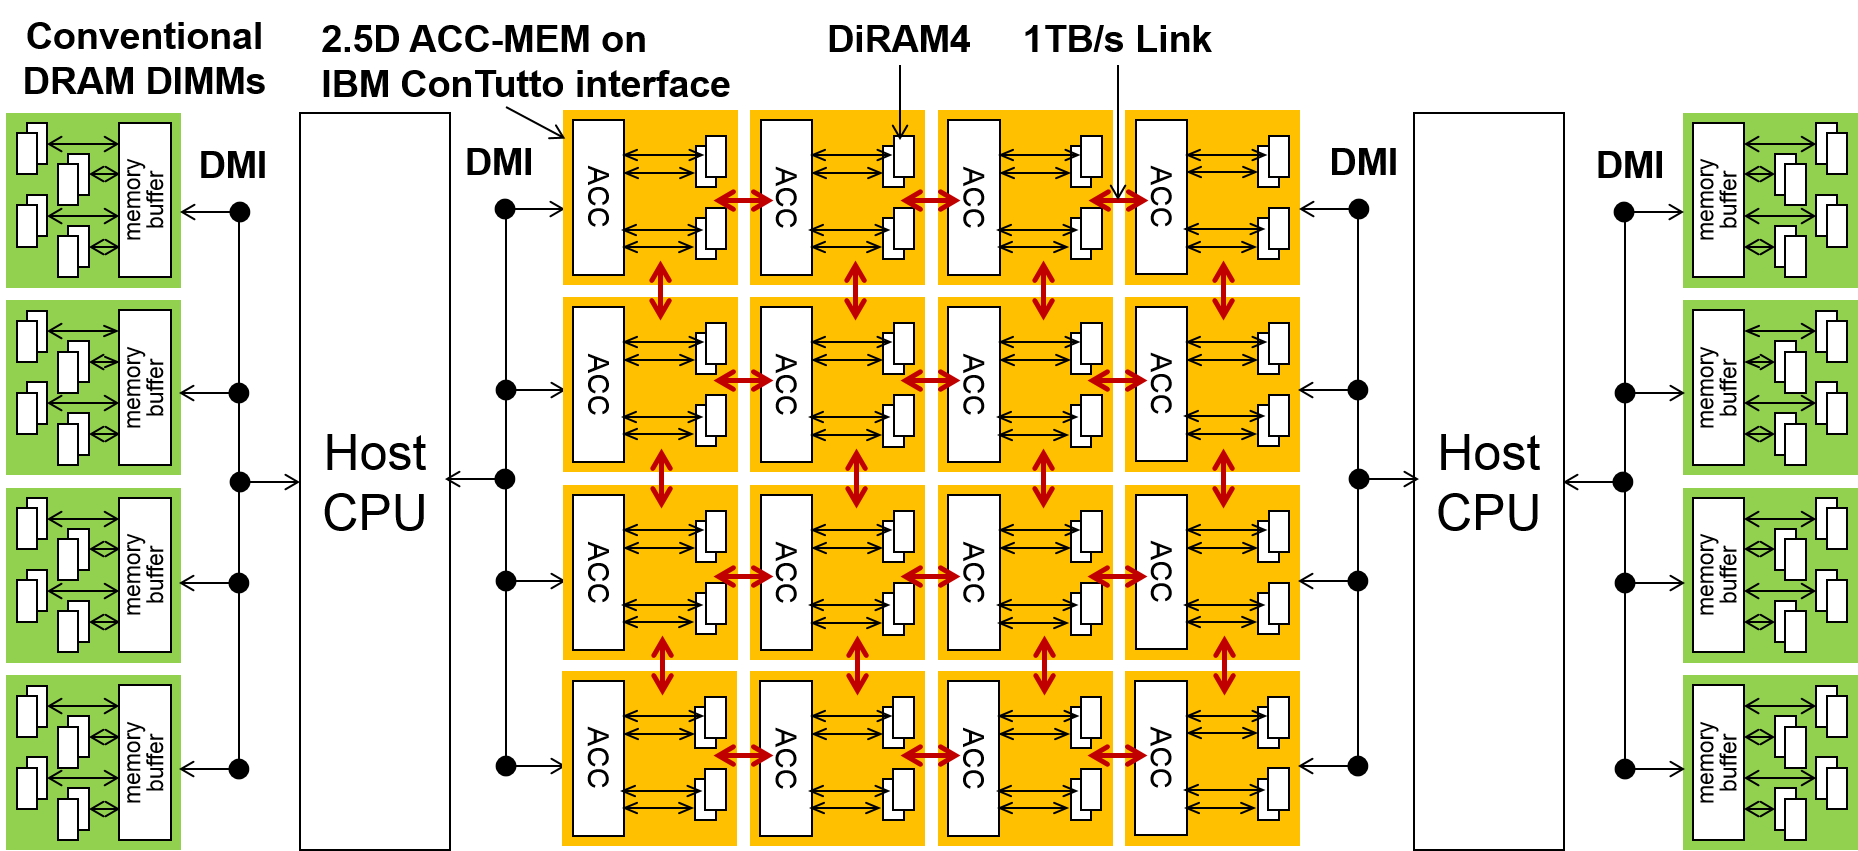
\includegraphics[width=1.0\linewidth]{fig/arch.png}
\caption{GAMA System Architecture}
\label{fig:arch}
\end{figure}
 



%the memory channel provides the highest bandwidth with the lowest latency amongst off-chip communication interfaces in contemporary computer systems.

 
 %Specifically,  a DiRAM4 die provides the same aggregate bandwidth as HBM2, but it provides 4X more channels than HBM2 where each channel supports only a quarter of the width of HBM2. We believe that DiRAM4 design is better suited for graph analytics where multiple accesses are made to random 


High bandwidth memory (HBM) and hybrid memory cube (HMC) used for recent PIM architectures can provide high bandwidth only for sequential, regular memory accesses. In contrast, graph analytics require efficient support for irregular and small granularity memory accesses. We tackle this problem by adopting a recent DiRAM4 3D Memory from Tezzaron and architecting on-chip caches and a custom memory controller to efficiently support small granularity irregular memory accesses. 
Specifically, DiRAM4 provides the same aggregate bandwidth as HBM2, but it provides 4X more (but narrower) channels than HBM2

.  The tiled architecture is built  

In this project, we envision to develop a PIM system depicted in Figure~\ref{fig:arch}. 
Overall, the system consists of a 16-node accelerator-memory (AM) cluster and IBM POWER8-based host systems.
An AM cluster is comprised of 16 nodes (packages) connected by our power-efficient high-bandwidth chip-to-chip links in a mesh style. 
One accelerator (ACC) and four 8GB DiRAM4 dies will constitute a PIM package with 4TB/s aggregate in-package bandwidth. 
%Our ACC die will integrate 16 ACCs with our custom eDRAM-based large shared and SRAM-based private on-chip cache, a 16$\times$16 crossbar, and a network interface (NI) to support chip-to-chip communications.

\begin{wrapfigure}{r}[0pt]{0.6\textwidth}
\center
%\vspace{-8ex}
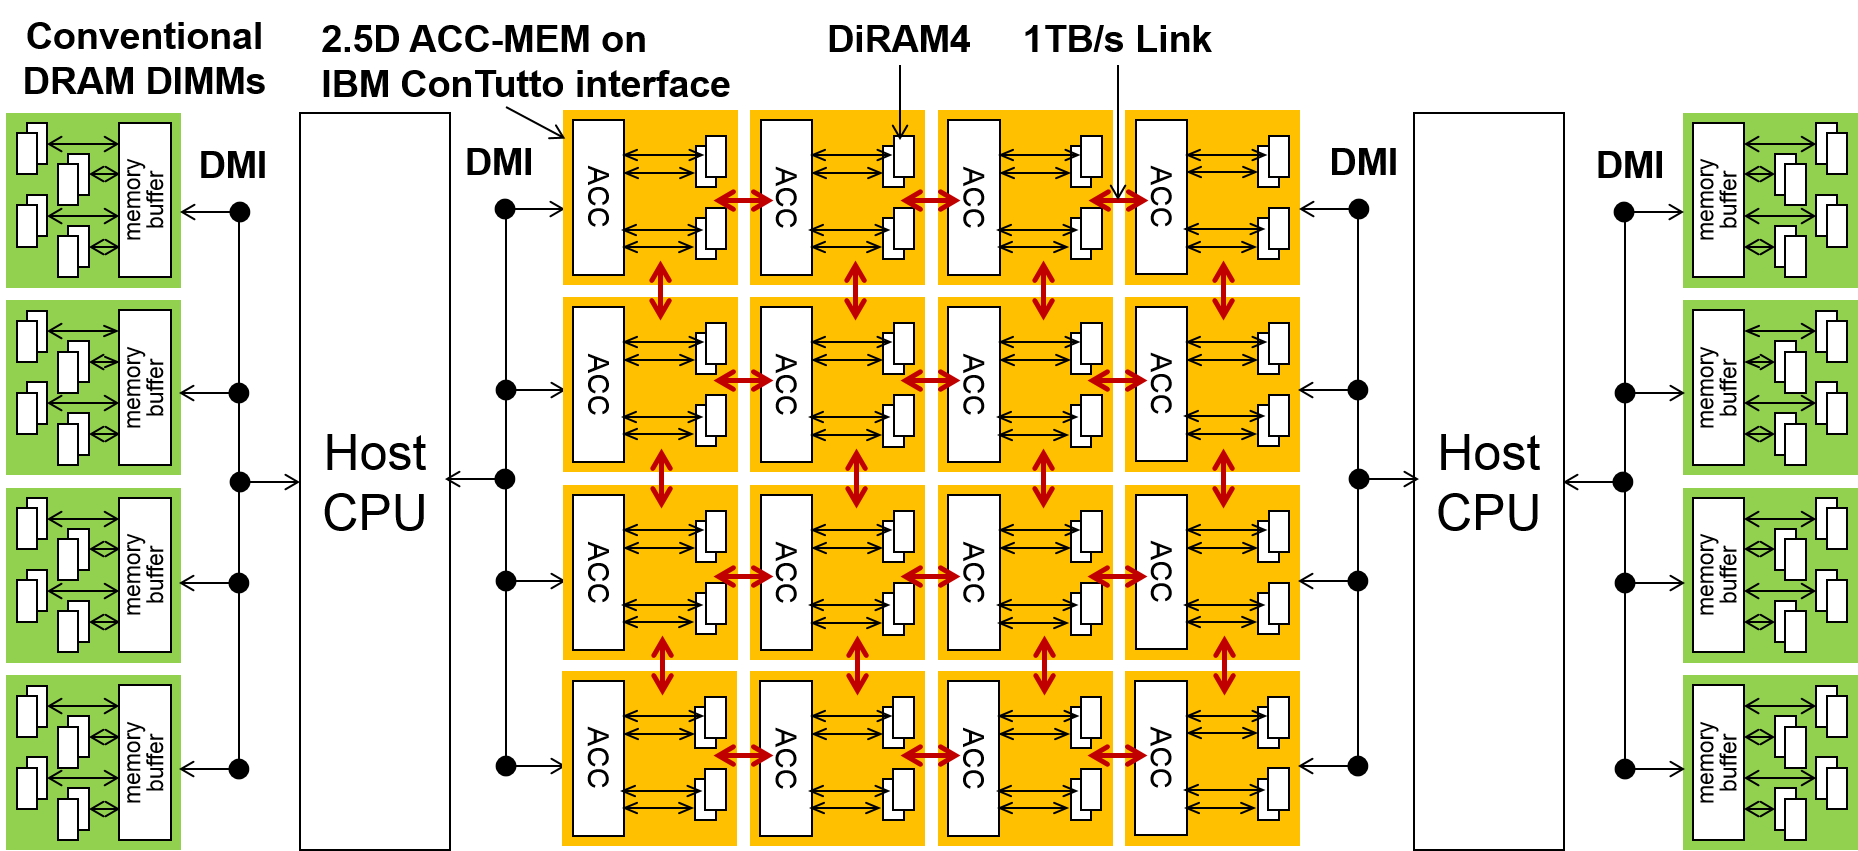
\includegraphics[width=1.0\linewidth]{./fig/arch.png}
\caption{The overall architecture of an Accelerator-Memory HIVE.}
\label{fig:arch}
\end{wrapfigure}

In the proposed PIM system, we propose to connect each AM packages to a memory channel of a host CPU providing 8 memory channels;
the memory channel provides the highest bandwidth with the lowest latency amongst off-chip communication interfaces in contemporary computer systems.
A IBM's ConTutto facilitates the interface between an AM package and the IBM's proprietary memory interface (DMI).
The memory space associated with the AM cluster is a non-cacheable region to eliminate the need for managing cache coherence between caches of the host systems and the AM HIVE.
The host system allocates the memory space of the AM cluster as a sinlge, continuous, and large physical memory segment which is preferred by big-data applications~\footnote{}.
ACCs are memory-mapped to part of the non-cacheable regions (as other I/O devices).

% Some notes
% We need a custom POWER8 board
\end{comment}
